% answers.tex —— 1977 年·广西百色卷（理科） · 参考答案与详细解析片段
% 由 tools/generate_projects.py 依来源总账自 1977/1977_数学真题_广西百色理_试题.md + 1977/1977_数学真题_广西百色理_解析正文.md + 1977/1977_数学真题_广西百色理_答案要点.md 生成，勿手改（改源 MD 后重跑）


\begin{gktip}
固定源是题面与解答连排的书籍材料（书页 141—146）。下文逐题独立推导，并与源解答对照复算：第 1—4、6 题与参考题的最终结论与源解答一致；第 2（1）题源解答把一般式一行误印作「x + 3y - 2 = 0」，与其自列的斜截式 $y=-\frac13x+2$ 矛盾，正确应为 $x+3y-6=0$，已在该题加源注；第 5 题题面第一式按源卷排印保留「cosc」（应读作角 $C$ 的余弦），源证明「同理可证」一行排印潦草（印作「b = CcoeA + acosC」样式），亦系排印之误，不影响题意。原卷无分值标注；卷末「选作题」两题本库按参考题 1、2 处理，解析接于第 6 题之后。
\end{gktip}

\begin{answer}
\gksolhead{1}{}

\textbf{题目}：

（1） 求函数 $y=\dfrac{2\sqrt{5-x}}{\sqrt{x-3}}$ 的定义域。

\Needspace{5\baselineskip}
（2） 计算：

\nopagebreak[4]
\[
\left(-\frac12\right)^{-3}+32^{\frac25}+5^0-3^{-2}
\]

（3） 求 $\sin^2 60^\circ+\operatorname{ctg}45^\circ+\dfrac34\operatorname{tg}^2 30^\circ-\cos 60^\circ$ 的值。

（4） $\log_2\sqrt8=x$，求 $x$。

\Needspace{4\baselineskip}
\textbf{解析}

\gksubpart{（1）}

\Needspace{5\baselineskip}
要使函数有意义，需根号内非负，且分母根号内严格为正：

\nopagebreak[4]
\[
5-x\ge0,
\qquad
x-3>0,
\]

\Needspace{5\baselineskip}
即 $x\le5$ 且 $x>3$。故定义域为

\nopagebreak[4]
\[
3<x\le5.
\]

\gksubpart{（2）}

\nopagebreak[4]
\[
\begin{aligned}
\left(-\frac12\right)^{-3}+32^{\frac25}+5^0-3^{-2}
&=(-2)^3+(2^5)^{\frac25}+1-\frac1{3^2}\\
&=-8+4+1-\frac19\\
&=-3\frac19.
\end{aligned}
\]

\gksubpart{（3）}

\nopagebreak[4]
\[
\begin{aligned}
\text{\text{原式}}
&=\left(\frac{\sqrt3}{2}\right)^2+1+\frac34\left(\frac{\sqrt3}{3}\right)^2-\frac12\\
&=\frac34+1+\frac14-\frac12=1\frac12.
\end{aligned}
\]

\gksubpart{（4）}

\Needspace{5\baselineskip}
$\log_2\sqrt8=x$ 即 $2^x=\sqrt8$。而 $\sqrt8=8^{\frac12}=2^{\frac32}$，故

\nopagebreak[4]
\[
x=\frac32.
\]

\gkanswer{答案（1）：$3<x\le5$。}

\gkanswer{答案（2）：$-3\dfrac19$。}

\gkanswer{答案（3）：$1\dfrac12$。}

\gkanswer{答案（4）：$x=\dfrac32$。}

\end{answer}
\begin{answer}
\gksolhead{2}{}

\textbf{题目}：

已知直线过 $(3,1)$ 和 $(-6,4)$ 两点。

（1） 求出这直线方程。

（2） 求它的斜率和 $y$ 轴上的截距。

（3） 这函数是上升或下降。

（4） 求过 $(0,-5)$ 和这直线平行的直线方程。

\Needspace{4\baselineskip}
\textbf{解析}

\gksubpart{（1）}

\Needspace{5\baselineskip}
设所求直线为 $y=kx+b$。把 $(3,1)$、$(-6,4)$ 代入：

\nopagebreak[4]
\[
\begin{cases}
1=3k+b,\\
4=-6k+b.
\end{cases}
\]

\Needspace{5\baselineskip}
两式相减得 $9k=-3$，即 $k=-\dfrac13$；代回第一式得 $b=1-3k=2$。故

\nopagebreak[4]
\[
y=-\frac13x+2,
\qquad\text{\text{即}}\qquad
x+3y-6=0.
\]

\begin{gktip}
\textbf{源注}：源解答把一般式一行印作「x + 3y - 2 = 0」，与其自列的斜截式 $y=-\dfrac13x+2$ 矛盾（把 $(3,1)$ 代入「x + 3y - 2」左端得 $4\ne0$）；按斜截式去分母应得 $x+3y-6=0$（把 $(3,1)$、$(-6,4)$ 代入验证均成立）。系排印之误，本文按复算结果收尾。
\end{gktip}

\gksubpart{（2）}

斜率为 $k=-\dfrac13$；在 $y=-\dfrac13x+2$ 中令 $x=0$，得 $y$ 轴上的截距为 $2$。

\gksubpart{（3）}

因为 $k=-\dfrac13<0$，所以这函数是下降的（$y$ 随 $x$ 的增大而减小）。

\gksubpart{（4）}

\Needspace{5\baselineskip}
平行直线的斜率相等，故所求直线的斜率也是 $-\dfrac13$；它过点 $(0,-5)$，即 $y$ 轴上的截距为 $-5$，故

\nopagebreak[4]
\[
y=-\frac13x-5,
\qquad\text{\text{即}}\qquad
x+3y+15=0.
\]

\gkanswer{答案（1）：$y=-\dfrac13x+2$，即 $x+3y-6=0$。}

\gkanswer{答案（2）：斜率为 $-\dfrac13$，$y$ 轴上的截距为 $2$。}

\gkanswer{答案（3）：这函数是下降的。}

\gkanswer{答案（4）：$y=-\dfrac13x-5$，即 $x+3y+15=0$。}

\end{answer}
\begin{answer}
\gksolhead{3}{}

\textbf{题目}：

已知圆 $O$ 中两弦 $AB$、$CD$ 相交于 $E$。

（1） 证明 $AE\cdot BE=CE\cdot DE$。

（2） 当 $CD$ 为直径（$2R$），$AB\perp CD$ 时，证明 $BE^2=CE(2R-CE)$。

\begin{gktip}
原源 PDF 第 3 页在本题旁附有圆内两弦相交示意图；LaTeX 版按源图重绘。
\end{gktip}
\nopagebreak[4]
\begin{center}% 1977 年广西百色卷（理科）第三题：圆 O 内两弦 AB、CD 相交于 E，
% 虚线 AC、BD 为证 △AEC∽△DEB 所连（按源卷第 3 页布局）
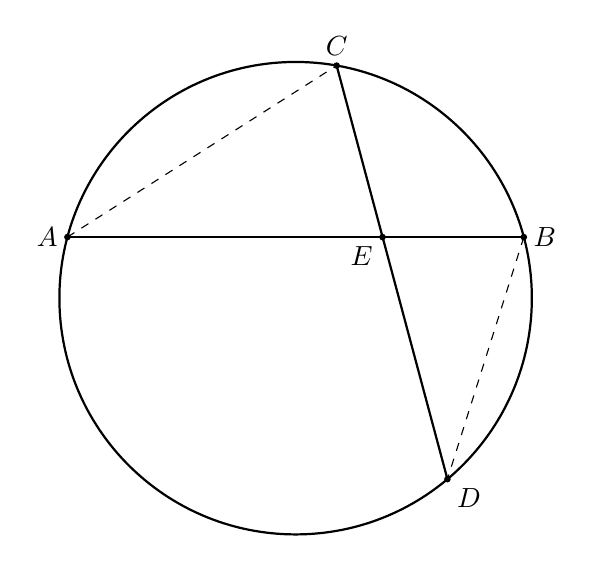
\begin{tikzpicture}[scale=1.0]
  % 圆半径 3cm；A 在 165°、B 在 15°、C 在 80°、D 在 310°
  \draw[thick] (0,0) circle (3);
  \coordinate (A) at (-2.898,0.776);
  \coordinate (B) at (2.898,0.776);
  \coordinate (C) at (0.521,2.954);
  \coordinate (D) at (1.928,-2.298);
  \coordinate (E) at (1.104,0.776); % AB 与 CD 的交点
  \draw[thick] (A)--(B);
  \draw[thick] (C)--(D);
  \draw[dashed] (A)--(C);
  \draw[dashed] (B)--(D);
  \fill (A) circle (1.2pt) node[left] {$A$};
  \fill (B) circle (1.2pt) node[right] {$B$};
  \fill (C) circle (1.2pt) node[above] {$C$};
  \fill (D) circle (1.2pt) node[below right] {$D$};
  \fill (E) circle (1.2pt) node[below left] {$E$};
\end{tikzpicture}
\end{center}
\nopagebreak[4]
\Needspace{4\baselineskip}
\textbf{解析}
\nopagebreak[4]
\begin{center}% 1977 年广西百色卷（理科）第三题：圆 O 内两弦 AB、CD 相交于 E，
% 虚线 AC、BD 为证 △AEC∽△DEB 所连（按源卷第 3 页布局）
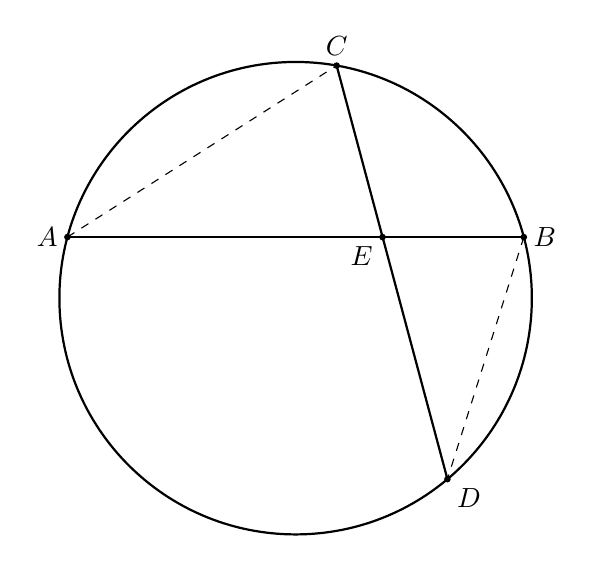
\begin{tikzpicture}[scale=1.0]
  % 圆半径 3cm；A 在 165°、B 在 15°、C 在 80°、D 在 310°
  \draw[thick] (0,0) circle (3);
  \coordinate (A) at (-2.898,0.776);
  \coordinate (B) at (2.898,0.776);
  \coordinate (C) at (0.521,2.954);
  \coordinate (D) at (1.928,-2.298);
  \coordinate (E) at (1.104,0.776); % AB 与 CD 的交点
  \draw[thick] (A)--(B);
  \draw[thick] (C)--(D);
  \draw[dashed] (A)--(C);
  \draw[dashed] (B)--(D);
  \fill (A) circle (1.2pt) node[left] {$A$};
  \fill (B) circle (1.2pt) node[right] {$B$};
  \fill (C) circle (1.2pt) node[above] {$C$};
  \fill (D) circle (1.2pt) node[below right] {$D$};
  \fill (E) circle (1.2pt) node[below left] {$E$};
\end{tikzpicture}
\end{center}
\nopagebreak[4]
\gksubpart{（1）}

\Needspace{5\baselineskip}
连结 $AC$、$BD$。在 $\triangle AEC$ 与 $\triangle DEB$ 中：$\angle AEC$ 与 $\angle DEB$ 是对顶角，故相等；$\angle EAC$ 与 $\angle EDB$ 是同弧 $CB$ 上的圆周角，故相等。于是

\nopagebreak[4]
\[
\triangle AEC\sim\triangle DEB
\quad\Longrightarrow\quad
\frac{AE}{DE}=\frac{CE}{BE},
\]

\Needspace{5\baselineskip}
整理即得

\nopagebreak[4]
\[
AE\cdot BE=CE\cdot DE.
\]

\gksubpart{（2）}

\Needspace{5\baselineskip}
因为 $CD$ 是直径且 $AB\perp CD$，由垂径定理（垂直于弦的直径平分弦），$AE=BE$；又 $D$ 在直径 $CD$ 上，故 $DE=CD-CE=2R-CE$。把两式代入（1）的结论

\nopagebreak[4]
\[
AE\cdot BE=CE\cdot DE
\]

\Needspace{5\baselineskip}
得

\nopagebreak[4]
\[
BE^2=CE(2R-CE).
\]

\gkanswer{答案（1）：见解析版}

\gkanswer{答案（2）：见解析版}

\end{answer}
\begin{answer}
\gksolhead{4}{}

\textbf{题目}：

一船往返于 $48$ 公里的两地，共航行 $10$ 小时，已知水流速度是 $2$ 公里/小时，求这轮船在静水中航行的速度。

\Needspace{4\baselineskip}
\textbf{解析}

\Needspace{5\baselineskip}
设轮船在静水中航行的速度为每小时 $x$ 公里（$x>2$，否则逆水速度非正）。则顺水速度为每小时 $(x+2)$ 公里，逆水速度为每小时 $(x-2)$ 公里。往返共航行 $10$ 小时：

\nopagebreak[4]
\[
\frac{48}{x+2}+\frac{48}{x-2}=10.
\]

\Needspace{5\baselineskip}
两边同乘 $(x+2)(x-2)$：

\nopagebreak[4]
\[
48(x-2)+48(x+2)=10(x^2-4),
\]

\nopagebreak[4]
\[
96x=10x^2-40,
\qquad
5x^2-48x-20=0,
\]

\nopagebreak[4]
\[
(5x+2)(x-10)=0.
\]

解得 $x=10$ 或 $x=-\dfrac25$。两根都使所乘整式不为零，但负速度不合题意，舍去 $x=-\dfrac25$。故轮船在静水中航行的速度是 $10$ 公里/小时。

\gkanswer{答案：$10$ 公里/小时。}

\end{answer}
\begin{answer}
\gksolhead{5}{}

\textbf{题目}：

\Needspace{5\baselineskip}
已知 $A$、$B$、$C$ 是 $\triangle ABC$ 的三个内角，求证

\nopagebreak[4]
\[
\begin{aligned}
&a=b\cos c+c\cos B,\\
&b=c\cos A+a\cos C,\\
&c=a\cos B+b\cos A.
\end{aligned}
\]

\begin{gktip}
\textbf{源注}：源卷把第一式余弦的角排印为小写「c」（印作「a = bcosc + ccosB」），系排印之误，此处保留转录，应读作 $\cos C$。求证的三条式子跨源卷第 4—5 页连排。
原源 PDF 第 4 页在本题旁附有三角形与底边上的高示意图；LaTeX 版按源图重绘。
\end{gktip}
\nopagebreak[4]
\begin{center}% 1977 年广西百色卷（理科）第五题：三角形 ABC 的三边 a、b、c，
% AD 为 BC 边上的高（虚线）（按源卷第 4 页布局）
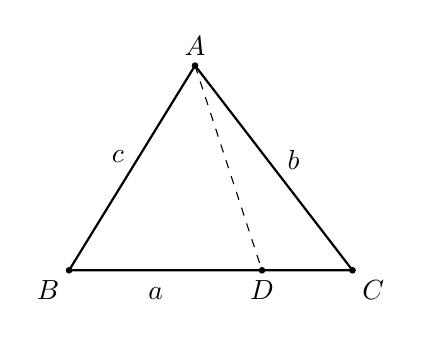
\begin{tikzpicture}[scale=1.0]
  \coordinate (A) at (1.6,2.6);
  \coordinate (B) at (0,0);
  \coordinate (C) at (3.6,0);
  \coordinate (D) at (2.45,0); % 高的垂足
  \draw[thick] (A)--(B)--(C)--cycle;
  \draw[dashed] (A)--(D);
  \fill (A) circle (1.2pt) node[above] {$A$};
  \fill (B) circle (1.2pt) node[below left] {$B$};
  \fill (C) circle (1.2pt) node[below right] {$C$};
  \fill (D) circle (1.2pt) node[below] {$D$};
  \node at (0.62,1.45) {$c$};
  \node at (2.85,1.40) {$b$};
  \node at (1.10,-0.30) {$a$};
\end{tikzpicture}
\end{center}
\nopagebreak[4]
\Needspace{4\baselineskip}
\textbf{解析}
\nopagebreak[4]
\begin{center}% 1977 年广西百色卷（理科）第五题：三角形 ABC 的三边 a、b、c，
% AD 为 BC 边上的高（虚线）（按源卷第 4 页布局）
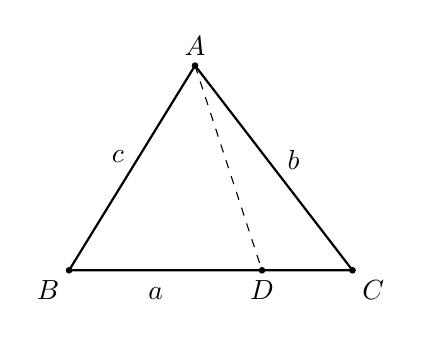
\begin{tikzpicture}[scale=1.0]
  \coordinate (A) at (1.6,2.6);
  \coordinate (B) at (0,0);
  \coordinate (C) at (3.6,0);
  \coordinate (D) at (2.45,0); % 高的垂足
  \draw[thick] (A)--(B)--(C)--cycle;
  \draw[dashed] (A)--(D);
  \fill (A) circle (1.2pt) node[above] {$A$};
  \fill (B) circle (1.2pt) node[below left] {$B$};
  \fill (C) circle (1.2pt) node[below right] {$C$};
  \fill (D) circle (1.2pt) node[below] {$D$};
  \node at (0.62,1.45) {$c$};
  \node at (2.85,1.40) {$b$};
  \node at (1.10,-0.30) {$a$};
\end{tikzpicture}
\end{center}
\nopagebreak[4]
\Needspace{5\baselineskip}
记 $a=BC$、$b=CA$、$c=AB$，作 $AD\perp BC$，垂足为 $D$。在直角 $\triangle ABD$ 中，

\nopagebreak[4]
\[
BD=AB\cos B=c\cos B;
\]

\Needspace{5\baselineskip}
在直角 $\triangle ACD$ 中，

\nopagebreak[4]
\[
DC=AC\cos C=b\cos C.
\]

\Needspace{5\baselineskip}
两段相加：

\nopagebreak[4]
\[
a=BC=BD+DC=c\cos B+b\cos C,
\]

即求证的第一式（题面按源卷排印把角 $C$ 印作小写）。作 $AC$ 边上的高，同理可证第二式 $b=c\cos A+a\cos C$；作 $AB$ 边上的高，同理可证第三式 $c=a\cos B+b\cos A$。

\gkanswer{答案：见解析版}

\end{answer}
\begin{answer}
\gksolhead{6}{}

\textbf{题目}：

当 $a$、$b$、$c$ 为实数时，求证方程 $x^2-(a+b)x+(ab-c^2)=0$ 有两个实数根，并求出两个根相等的条件。

\begin{gktip}
\textbf{参考题说明}：源卷第六题后印有「选作题：」栏，其下两题以「1、」「2、」编号。本库按参考题 1、2 处理，不计入正式题量。
\end{gktip}

\Needspace{5\baselineskip}
\textbf{参考题 1．} 已知：

\nopagebreak[4]
\[
2\lg(x-2y)=\lg x+\lg y,
\]

求：$x:y$。

\textbf{参考题 2．} 求内接于半径为 $10$ 厘米，圆心角为 $120^\circ$ 的弓形的正方形的边长。

\begin{gktip}
原源 PDF 第 6 页在本题旁附有弓形内接正方形示意图；LaTeX 版按源图重绘。
\end{gktip}
\nopagebreak[4]
\begin{center}% 1977 年广西百色卷（理科）参考题 2（源卷「选作题」第 2 题）：半径 10cm、
% 圆心角 120° 的弓形内接正方形 CDEF，半径 OP⊥FE 交 FE 于 N、AB 于 M（按源卷第 6 页布局）
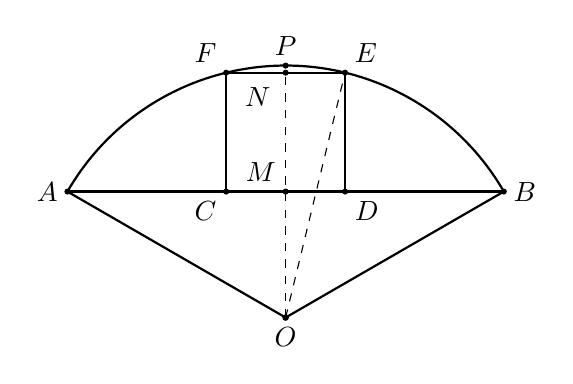
\begin{tikzpicture}[scale=1.0]
  % O 为圆心，R=3.2cm；A、B 为弦端点，C、D 在弦上，F、E 在弧上，P 为弧中点
  \coordinate (O) at (0,0);
  \coordinate (A) at (-2.771,1.6);
  \coordinate (B) at (2.771,1.6);
  \coordinate (M) at (0,1.6);
  \coordinate (C) at (-0.755,1.6);
  \coordinate (D) at (0.755,1.6);
  \coordinate (N) at (0,3.110);
  \coordinate (F) at (-0.755,3.110);
  \coordinate (E) at (0.755,3.110);
  \coordinate (P) at (0,3.2);
  \draw[thick] (O)--(A);
  \draw[thick] (O)--(B);
  \draw[thick] (A)--(B);
  \draw[thick] (A) arc (150:30:3.2);
  \draw[thick] (C)--(F)--(E)--(D);
  \draw[dashed] (O)--(P);
  \draw[dashed] (O)--(E);
  \fill (O) circle (1.2pt) node[below] {$O$};
  \fill (A) circle (1.1pt) node[left] {$A$};
  \fill (B) circle (1.1pt) node[right] {$B$};
  \fill (P) circle (1.1pt) node[above] {$P$};
  \fill (F) circle (1.1pt) node[above left] {$F$};
  \fill (E) circle (1.1pt) node[above right] {$E$};
  \fill (C) circle (1.1pt) node[below left] {$C$};
  \fill (D) circle (1.1pt) node[below right] {$D$};
  \fill (M) circle (1.1pt) node[above left] {$M$};
  \fill (N) circle (1.1pt) node[below left=2pt] {$N$};
\end{tikzpicture}
\end{center}
\nopagebreak[4]
\Needspace{4\baselineskip}
\textbf{解析}

\Needspace{5\baselineskip}
判别式

\nopagebreak[4]
\[
\begin{aligned}
\Delta&=[-(a+b)]^2-4\times1\times(ab-c^2)\\
&=a^2+2ab+b^2-4ab+4c^2\\
&=(a-b)^2+4c^2.
\end{aligned}
\]

\Needspace{5\baselineskip}
当 $a$、$b$、$c$ 为实数时，$(a-b)^2\ge0$、$4c^2\ge0$，故 $\Delta\ge0$ 恒成立，方程必有两个实数根。两根相等当且仅当 $\Delta=0$；而两个非负项之和为零当且仅当每项为零，即

\nopagebreak[4]
\[
a=b,
\qquad
c=0.
\]

故两根相等的条件是 $a=b$ 且 $c=0$。

\textbf{参考题 1}

\Needspace{5\baselineskip}
由对数性质，须 $x>0$、$y>0$ 且 $x-2y>0$。原方程左端即 $\lg(x-2y)^2$，右端 $\lg x+\lg y=\lg(xy)$，故

\nopagebreak[4]
\[
(x-2y)^2=xy,
\]

\nopagebreak[4]
\[
x^2-5xy+4y^2=0,
\qquad
(x-4y)(x-y)=0.
\]

\Needspace{5\baselineskip}
若 $x=y$，则 $x-2y=-y<0$，不合；若 $x=4y$，则 $x-2y=2y>0$，合题意。故

\nopagebreak[4]
\[
x:y=4.
\]

\textbf{参考题 2}
\nopagebreak[4]
\begin{center}% 1977 年广西百色卷（理科）参考题 2（源卷「选作题」第 2 题）：半径 10cm、
% 圆心角 120° 的弓形内接正方形 CDEF，半径 OP⊥FE 交 FE 于 N、AB 于 M（按源卷第 6 页布局）
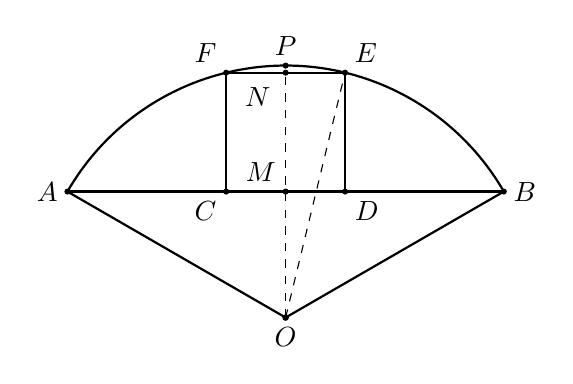
\begin{tikzpicture}[scale=1.0]
  % O 为圆心，R=3.2cm；A、B 为弦端点，C、D 在弦上，F、E 在弧上，P 为弧中点
  \coordinate (O) at (0,0);
  \coordinate (A) at (-2.771,1.6);
  \coordinate (B) at (2.771,1.6);
  \coordinate (M) at (0,1.6);
  \coordinate (C) at (-0.755,1.6);
  \coordinate (D) at (0.755,1.6);
  \coordinate (N) at (0,3.110);
  \coordinate (F) at (-0.755,3.110);
  \coordinate (E) at (0.755,3.110);
  \coordinate (P) at (0,3.2);
  \draw[thick] (O)--(A);
  \draw[thick] (O)--(B);
  \draw[thick] (A)--(B);
  \draw[thick] (A) arc (150:30:3.2);
  \draw[thick] (C)--(F)--(E)--(D);
  \draw[dashed] (O)--(P);
  \draw[dashed] (O)--(E);
  \fill (O) circle (1.2pt) node[below] {$O$};
  \fill (A) circle (1.1pt) node[left] {$A$};
  \fill (B) circle (1.1pt) node[right] {$B$};
  \fill (P) circle (1.1pt) node[above] {$P$};
  \fill (F) circle (1.1pt) node[above left] {$F$};
  \fill (E) circle (1.1pt) node[above right] {$E$};
  \fill (C) circle (1.1pt) node[below left] {$C$};
  \fill (D) circle (1.1pt) node[below right] {$D$};
  \fill (M) circle (1.1pt) node[above left] {$M$};
  \fill (N) circle (1.1pt) node[below left=2pt] {$N$};
\end{tikzpicture}
\end{center}
\nopagebreak[4]
\Needspace{5\baselineskip}
设正方形边长为 $x$ 厘米。作半径 $OP\perp FE$，交 $FE$ 于 $N$、$AB$ 于 $M$，连结 $OE$。由对称性，$OP$ 平分弦 $FE$ 与 $AB$，也平分圆心角 $\angle AOB$。在直角 $\triangle OMB$ 中，$\angle BOM=\dfrac{120^\circ}{2}=60^\circ$，$OB=10$，故

\nopagebreak[4]
\[
OM=10\cos60^\circ=10\times\frac12=5.
\]

\Needspace{5\baselineskip}
$MN$ 等于正方形的边长 $x$，$NE=\dfrac x2$（$OP$ 平分 $FE$），故 $ON=OM+MN=5+x$。在直角 $\triangle ONE$ 中，$OE=10$，由勾股定理：

\nopagebreak[4]
\[
(5+x)^2+\left(\frac x2\right)^2=10^2,
\]

\nopagebreak[4]
\[
x^2+8x-60=0,
\qquad
x=-4\pm2\sqrt{19}.
\]

\Needspace{5\baselineskip}
负根不合题意，舍去；取正根

\nopagebreak[4]
\[
x=-4+2\sqrt{19}\approx4.7.
\]

故内接于半径为 $10$ 厘米、圆心角为 $120^\circ$ 的弓形的正方形边长约为 $4.7$ 厘米。

\gkanswer{答案：方程恒有两个实数根；两根相等的条件是 $a=b$ 且 $c=0$。}

\end{answer}